% ITY: Projekt 2, Andrej Barna (xbarna01), 2014/2015
\documentclass[11pt,a4paper]{article}
\usepackage[left=2cm,text={17cm, 24cm},top=3cm]{geometry}
\usepackage{times}
\usepackage[czech]{babel}
\usepackage[utf8]{inputenc}
\usepackage[T1]{fontenc}
\usepackage{array}
\usepackage{multirow}
\usepackage{graphics}
\usepackage[czech,ruled,linesnumbered,noline,longend]{algorithm2e}
\providecommand{\uv}[1]{„#1“}


\begin{document}
\begin{titlepage}
\begin{center}
\Huge
\textsc{Vysoké učení technické v~Brně\\
\huge Fakulta informačních technologií}\\
\vspace{\stretch{0.382}}
\LARGE Typografie a publikování\,--\,3. projekt\\
\Huge Tabulky a~obrázky
\vspace{\stretch{0.618}}
\end{center}
\Large 6. dubna 2015\hfill Andrej Barna
\end{titlepage}


\section{Úvodní strana}
Název práce umístěte do zlatého řezu a nezapomeňte uvést dnešní datum a vaše jméno a příjmení.

\section{Tabulky}
Pro sázení tabulek můžeme použít buď prostředí \texttt{tabbing} nebo prostředí \texttt{tabular}.

\subsection{Prostředí \texttt{tabbing}}
Při použití \texttt{tabbing} vypadá tabulka následovně:

\begin{tabbing}
Vodní melouny \quad \= Cena \quad \= Množství\kill
\textbf{Ovoce} \> \textbf{Cena} \> \textbf{Množství}\\
Jablka \> 25,90 \> 3\,kg \\
Hrušky \> 27,40 \> 2,5\,kg \\
Vodní melouny \> 35,-- \> 1\,kus \\
\end{tabbing}
Toto prostředí se dá také použít pro sázení algoritmů, ovšem vhodnější je použít prostředí \texttt{algorithm} nebo \texttt{algorithm2e} (viz sekce 3).

\subsection{Prostředí \texttt{tabular}}
Další možností, jak vytvořit tabulku, je použít prostředí \texttt{tabular}. Tabulky pak budou vypadat takto\footnote{Kdyby byl problem s~\texttt{cline}, zkuste se podívat třeba sem: http://www.abclinuxu.cz/tex/poradna/show/325037. }:
\begin{table}[ht]
 \catcode`\-=12
\begin{center}
\begin{tabular}{| l | r | r |} \hline
  & \multicolumn{2}{c |}{\textbf{Cena}} \\ \cline{2-3}
\textbf{Měna} & \textbf{nákup} & \textbf{prodej}\\ \hline
EUR & 27,34 & 27,42 \\
GPB & 33,09 & 33,21 \\
USD & 19,87 & 19,95 \\ \hline
\end{tabular}
\caption{Tabulka kurzů k~dnešnímu dni}
\label{tabKurzyDnes}
\end{center}
\end{table}
\begin{table}[h]
\catcode`\-=12
\begin{center}
\begin{tabular}{| >{\bfseries}c | c |}\hline
$A$ & $\neg A$ \\\hline
P & N \\\hline
O~& O~\\\hline
X & X \\\hline
N & P \\\hline
\end{tabular}
\begin{tabular}{| c | >{\bfseries}c | c | c | c | c |}\hline
\multicolumn{2}{|c|}{\multirow{2}{*}{$A\wedge B$}} & \multicolumn{4}{c|}{$B$} \\ \cline{3-6} 
\multicolumn{2}{|c|}{} & \bfseries P & \bfseries O~& \bfseries X & \bfseries N \\ \hline
\multirow{4}{*}{$A$}& P & P & O~& X & N \\ \cline{2-6} 
                               & O~& O~& O~& N & N \\ \cline{2-6} 
                               & X & X & N & X & N \\ \cline{2-6} 
                               & N & N & N & N & N \\ \hline
\end{tabular}
\begin{tabular}{| c | >{\bfseries}c | c | c | c | c |}\hline
\multicolumn{2}{|c|}{\multirow{2}{*}{$A\vee B$}} & \multicolumn{4}{c|}{$B$} \\ \cline{3-6} 
\multicolumn{2}{|c|}{} & \bfseries P & \bfseries O~& \bfseries X & \bfseries N \\ \hline
\multirow{4}{*}{$A$}& P & P & P & P & P \\ \cline{2-6} 
                               & O~& P & O~& P & O~\\ \cline{2-6} 
                               & X & P & P & X & X \\ \cline{2-6} 
                               & N & P & O~& X & N \\ \hline
\end{tabular}
\begin{tabular}{| c | >{\bfseries}c | c | c | c | c |}\hline
\multicolumn{2}{|c|}{\multirow{2}{*}{$A\rightarrow B$}} & \multicolumn{4}{c|}{$B$} \\ \cline{3-6} 
\multicolumn{2}{|c|}{} & \bfseries P & \bfseries O~& \bfseries X & \bfseries N \\ \hline
\multirow{4}{*}{$A$}& P & P & O~& X & N \\ \cline{2-6} 
                               & O~& P & O~& P & O~\\ \cline{2-6} 
                               & X & P & P & X & X \\ \cline{2-6} 
                               & N & P & P & P & P \\ \hline
\end{tabular}
\caption{Protože Kleeneho trojhodnotová logika už je \uv{zastaralá}, uvádíme si zde příklad čtyřhodnotové
logiky}
\label{tabLogiky}
\end{center}
 \end{table}
\section{Algoritmy}
Pokud budeme chtít vysázet algoritmus, můžeme použít prostředí \texttt{algorithm}\footnote{Pro nápovědu, jak zacházet s~prostředím \texttt{algorithm}, můžeme zkusit tuhle stránku:\\
http://ftp.cstug.cz/pub/tex/CTAN/macros/latex/contrib/algorithms/algorithms.pdf.} nebo \texttt{algorithm2e}\footnote{Pro \texttt{algorithm2e} zase tuhle: http://ftp.cstug.cz/pub/tex/CTAN/macros/latex/contrib/algorithm2e/doc/algorithm2e.pdf.}.
Příklad použití prostředí \texttt{algorithm2e} viz Algoritmus \ref{algFastSLAM}.
\begin{algorithm}
\label{algFastSLAM}
\SetNlSty{}{}{:}
\SetNlSkip{-1.1em}
\caption{\textsc{FastSLAM}}
\KwIn{($X_{t-1}$, $u_t$, $z_t$)}
\KwOut{$X_t$}
\Indp
$\overline{X_t} = X_t = 0$\\
\For{$k = 1\textnormal{ to } M$}{$x_t^{[k]} = sample\_motion\_model(u_t, x_{t-1}^{[k]})$\\
$\omega_t^{[k]} = measurement\_model(z_t, x_t^{[k]}, m_{t-1})$\\
$m_t^{[k]} = updated\_occupancy\_grid(z_t, x_t^{[k]}, m_{t-1}^{[k]})$\\
$\overline{X_t} = \overline{X_t} + \langle x_x^{[m]}, \omega_t^{[m]}\rangle$\\}
\For{$k = 1\textnormal{ to } M$}
{draw $i$ with probability $\approx\omega_t^{[i]}$\\
add $\langle x_x^{[k]}, m_t^{[k]}\rangle$ to $X_t$}
\KwRet{$X_t$}
\end{algorithm}
\section{Obrázky}
Do našich článků mužeme samozřejmě vkládat obrázky. Pokud je obrázkem fotografie, můžeme klidně použít
bitmapový soubor. Pokud by to ale mělo být nějaké schéma nebo něco podobného, je dobrým zvykem takovýto
obrázek vytvořit vektorově.

\begin{figure}[ht]
  \begin{center}
  \scalebox{0.4}{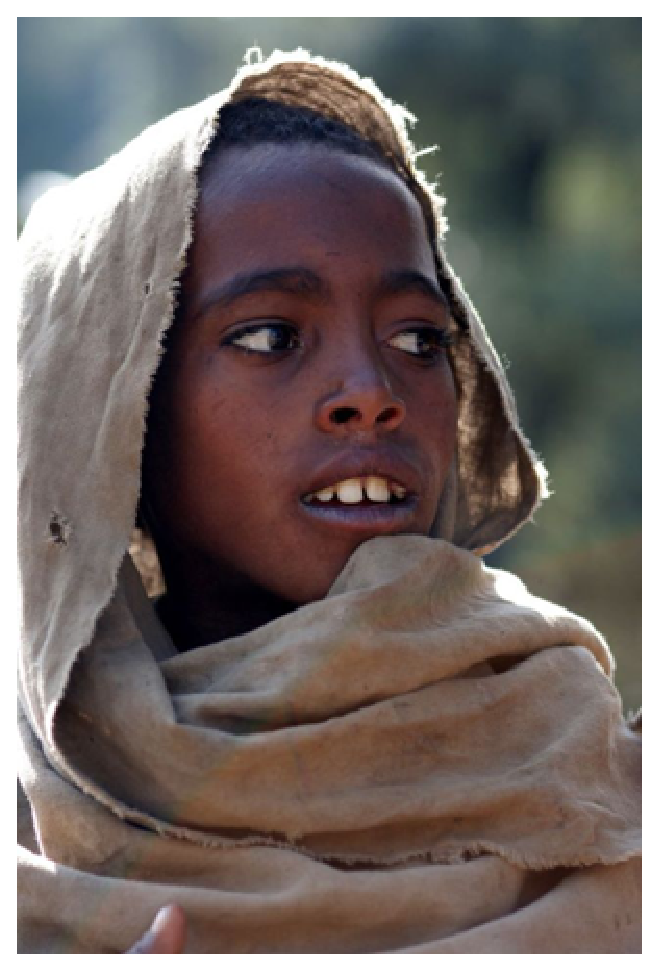
\includegraphics{etiopan.eps}
  \reflectbox{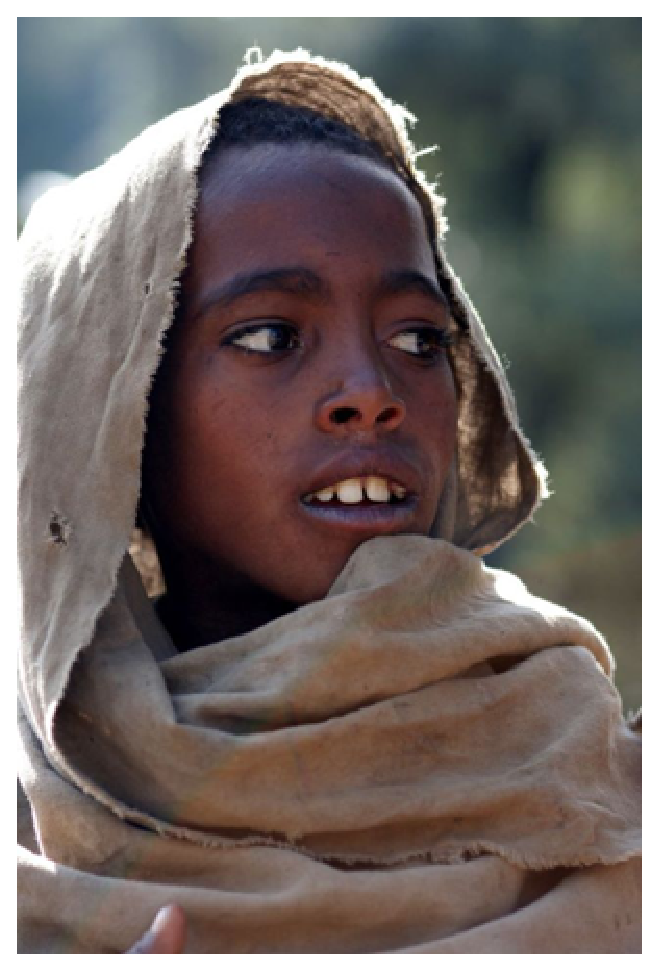
\includegraphics{etiopan.eps}}}
  \caption{Malý Etiopánek a jeho bratříček}
  \label{etiopiaboys}
  \end{center}
\end{figure}
Rozdíl mezi vektorovým\dots
\begin{figure}[ht]
  \begin{center}
  \scalebox{0.4}{
\includegraphics{oniisan.eps}}
  \caption{Vektorový obrázek}
  \label{oniisanvector}
  \end{center}
\end{figure}
\\\dots  a bitmapovým obrázkem
\begin{figure}[ht]
  \begin{center}
  \scalebox{0.6}{
\includegraphics{oniisan2.eps}}
  \caption{Bitmapový obrázek}
  \label{oniisanbitmap}
  \end{center}
\end{figure}
\\se projeví například při zvětšení.

Odkazy (nejen ty) na obrázky \ref{etiopiaboys}, \ref{oniisanvector} a \ref{oniisanbitmap}, na tabulky \ref{tabKurzyDnes} a \ref{tabLogiky} a také na algoritmus \ref{algFastSLAM} jsou udělány pomocí křížových odkazů. Pak je ovšem potřeba zdrojový soubor přeložit dvakrát.

Vektorové obrázky lze vytvořit i přímo v~\LaTeX u, například pomocí prostředí \texttt{picture}. Všechny rozměry
jsou uváděny v~mm.

\begin{figure}[ht]
  \setlength{\unitlength}{1.35mm}
  \begin{center}
  \begin{picture}(115,158.5)
  
  \linethickness{1pt}
  % Oramovanie  
    \put(0,0){\framebox(115,158.5){}}
  % Pata
    \put(30,10){\framebox(55,10){\textbf{Pata}}}
  % Textove telo
    \put(30,35){\framebox(55,75){\textbf{Textové tělo}}}
  % Okrajova poznamka
    \put(94,80){\framebox(15,10){\shortstack{\textbf{Okrajová}\\ \textbf{poznámka}}}}
  % Hlavicka
    \put(30,124){\framebox(55,10){\textbf{Hlavička}}}

  \linethickness{0.4pt}
  % Bocna sipka - vyska strany
    \put(112,79.25){\vector(0,1){79.25}}
    \put(112,79.25){\vector(0,-1){79.25}}
    \put(102,57){\vector(1,1){10}}
  % Sipka ''Vyska medzery'' 1
    \put(88,151.25){\vector(0,1){7.25}}
    \put(88,151.25){\vector(0,-1){7.25}}
  % Sipka ''Vyska medzery'' 2
    \put(88,139){\vector(0,1){5}}
    \put(88,139){\vector(0,-1){5}}
  % Sipka ''Vyska hlavicky''
    \put(88,129){\vector(0,1){5}}
    \put(88,129){\vector(0,-1){5}}
  % Sipka ''Vyska medzery'' 3
    \put(88,117){\vector(0,1){7}}
    \put(88,117){\vector(0,-1){7}}
  % Sipka ''Vyska tela''
    \put(88,72.5){\vector(0,1){37.5}}
    \put(88,72.5){\vector(0,-1){37.5}}
  % Sipka ''Vyska medzery'' 4
    \put(88,27.5){\vector(0,1){7.5}}
    \put(88,27.5){\vector(0,-1){7.5}}
  % Sipka ''Vyska paty''
    \put(88,15){\vector(0,1){5}}
    \put(88,15){\vector(0,-1){5}}
  
  % Spodna sipka - sirka strany
    \put(57.5,3){\vector(1,0){57.5}}
    \put(57.5,3){\vector(-1,0){57.5}}
  % Sipka ''Medzera'' 1
    \put(7.5,93){\vector(1,0){7.5}}
    \put(7.5,93){\vector(-1,0){7.5}}
  % Sipka ''Sirka boxu'' 1
    \put(57.5,137){\vector(1,0){27.5}}
    \put(57.5,137){\vector(-1,0){27.5}}
  % Sipka ''Medzera'' 2
    \put(89.5,93){\vector(1,0){4.5}}
    \put(89.5,93){\vector(-1,0){4.5}}
    \put(94.5,105){\vector(-1,-3){4}}
  % Sipka ''Sirka boxu'' 2
    \put(101.5,93){\vector(1,0){7.5}}
    \put(101.5,93){\vector(-1,0){7.5}}

  % Prerusovane ciary
    \multiput(0,144)(10,0){11}{\line(1,0){7}}
    \multiput(15,158.5)(0,-10){16}{\line(0,-1){7}}

  % Popisy ciar
    \put(7.5,95){\makebox(0,0){Mezera = 15}}
    \put(57.5,139){\makebox(0,0){Šířka boxu = 55}}
    \put(57.5,5){\makebox(0,0){Šířka stránky = 115}}
    \put(98.25,152){\makebox(0,0){\shortstack{Výška\\mezery = 14,5}}}
    \put(97.25,139){\makebox(0,0){\shortstack{Výška\\mezery = 10}}}
    \put(97.75,129){\makebox(0,0){\shortstack{Výška\\hlavičky = 10}}}
    \put(97,116.5){\makebox(0,0){\shortstack{Výška\\mezery = 14}}}
    \put(97.5,106.5){\makebox(0,0){Mezera = 9}}
    \put(102,96.5){\makebox(0,0){\shortstack{Šířka\\boxu = 15}}}
    \put(95,66){\makebox(0,0){\shortstack{Výška\\těla = 75}}}
    \put(102,52.5){\makebox(0,0){\shortstack{Výška\\stránky = 158,5}}}
    \put(97,27.5){\makebox(0,0){\shortstack{Výška\\mezery = 15}}}
    \put(95.5,14.5){\makebox(0,0){\shortstack{Výška\\paty = 10}}}
\end{picture}
\end{center}

\caption{Vektorový obrázek v~prostředí \texttt{picture}.}
\label{picpage}
\end{figure}
\end{document}
